%
%Documento dei requisiti per il sito @@@@@@@@@@
%Autore: Marco Pavan
%Versione 1.0
%
\documentclass[a4paper]{report}	%tipologia di documento

\usepackage[italian]{babel}	%pacchetto per la lingua italiana
%\usepackage[T1]{fontenc}	%da togliere se si compila con PDFLaTeX
\usepackage[utf8]{inputenc}	%per caratteri speciali (lettere accentate ecc...)
\usepackage{graphicx}		%per importare immagini
\frenchspacing			%spaziatura "alla francese" 
%\usepackage{hyperref}		%supporto per gestire i collegamenti e le url
%\usepackage{latexsym}		%inserimento di simboli di tipo matematico
%\usepackage{listings}		%inserimento di codice sorgente

\title{Documento dei Requisiti \\ per il sito: vinitricardi.it \\ \small{Versione 1.0}}		%titolo
\author{Marco Pavan - pavan.marco@email.it}		%autore
\date{\today}			%data di ultimo aggiornamento

\begin{document}		%inizio del documento

\maketitle			%inserimento del titolo

%\begin{abstract}		%eventuale abstract
%\end{abstract}

\newpage			%generazione delle prime pagine
\pagenumbering{roman}		%numerazione romana per le pagine iniziali
\tableofcontents		
\listoffigures
%\listoftables
\newpage

\section*{Introduzione}		%introduzione
\markboth{Introduzione}{Introduzione}
Il presente documento è redatto al fine di organizzare le informazioni raccolte attraverso le interviste fatte ai committenti per lo sviluppo del sito web dell'azienda ``Tricardi''.
Le informazioni qui raccolte hanno origine in parte dal committente, in parte da considerazioni ed analisi personali.
Il presente documento viene aggiornato ad ogni nuovo vincolo o requisito si presenti durante lo sviluppo o la manutenzione del sito, non deve essere considerato come fisso e immutabile ma, bensì, soggetto a continui aggiornamenti e revisioni.

\pagenumbering{arabic}
\chapter{Generalità}
\section{Il committente}I committenti sono: Alex Pintar (mdtricardi@gmail.it, 3273497406) e Stefano Catucciato, proprietari dell'azienda ``Vini Tricardi s.r.l.'' con sede in località Velerisce n. 7 34070 San Floriano del Collio (Gorizia). \\
L'azienda, a conduzione familiare, si occupa di commercio di vari prodotti della gastronomia italiana e della produzione e commercio di vini DOC friulani. Il sito \textit{www.vinitricardi.it} avrà, infatti, lo scopo di pubblicizzare e definire i contatti con la clientela proprio a supporto di quest'ultima attività.  
  
\section{Situazione attuale}
Esistono più siti web riferibili all'azienda Tricardi.\\ 
\textsl{www.tricardi.com} - di chiaro stampo commerciale, presenta una serie di prodotti a marchio Tricardi che spaziano dai vini alla birra, all'olio di oliva, al caffè\ldots E' un sito creato interamente con tecnologia Flash, di grande impatto visivo ma di scarsa incisività in quanto presenza sui motori di ricerca e visibilità Web.
\textsl{www.pintar.it} - presenta una carellata di vini a marchio Pintar e una breve descrizione dell'azienda Pintar. Anche in questo caso si ha scarsa attenzione riguardo alle tecnologie usate e il loro impatto riguardo la presenza sui motori di ricerca: il sito è stato creato impiegando dei frame HTML influendo, così, negativamente su usabilità, accessibilità e ottimizzazione dei contenuti. 

\section{Obiettivi generali del sito}
Il sito ha lo scopo di raggiungere determinati obiettivi, alcuni di carattere generale, altri più specifici. Si cerca di evidenziarne i principali dandone anche una valutazione circa la priorità. Gli obiettivi generali che il sito vuole ottenere sono:
\begin{itemize}
\item far conoscere l'azienda anche attraverso il Web	(priorità alta)
\item aumentare la popolarità del'azienda attraverso i motori di ricerca	(priorità alta)
\item fornire uno strumento di comunicazione tra i proprietari e i loro clienti 	(priorità alta)
\item fornire una descrizione dell'azienda attraverso foto e descrizioni testuali	(priorità media)
\item fornire tutte le informazioni per raggiungere l'azienda e per comunicare con i proprietari 	(priorità alta)
\item tenere i visitatori aggiornati sulle ultime novità o iniziative 	(priorità bassa)
\item fornire una serie di link utili 	(priorità bassa)
\end{itemize}
Più nello specifico, altri obiettivi sono:
\begin{itemize}
\item pubblicizzare i vini DOC a marchio Tricardi	(priorità alta)
\item permettere all'utente di scaricare le schede tecniche di ogni vino presente	(priorità alta)
\item informare su tecniche di produzione, qualità dei vini e prezzi	(priorità media)
\item fornire le indicazioni sopra riportate in più lingue	(priorità alta)
\end{itemize}

\section{Utenti}
\subsection{Utenti esterni}
Gli utenti che si vogliono raggiungere sono medi e grandi importatori, soprattutto esteri (in tal caso la disponibilità dei contenuti in lingua inglese è molto importante). Non si vuole raggiungere la clientela privata e neppure i servizi di ristorazione, ma il target è appunto la grande distribuzione.

\chapter{Requisiti del sito}
\section{Requisiti di architettura e contenuto}
Si analizza la struttura di navigazione del sito cercando di progettarla in modo coerente con la struttura informativa ed di renderla il più possibile intuitiva per l'utente che la utilizza. 
\subsection{Scaletta logica dei contenuti}
La scaletta logica descrive la struttura gerarchica dei contenuti nella sua strutturazione in sezioni e sottosezioni, ne specifica il nome (l'etichetta che comparirà come titolo per ogni sezione) e ne elenca i contenuti principali.
\begin{itemize}
\item \textbf{Home page} (testo introduttivo al sito, mail e contatti, link al sito "\textsl{www.tricardi.com}")
  \begin{itemize}
  \item \textbf{I nostri vini} (descrizione introduttiva e scheda tecnica per ogni vino presente)
  \item \textbf{L'azienda} (presentazione e breve storia dell'azienda)
  \item \textbf{FAQ} (risposte alle domande più frequenti riguardo l'azienda e la sua produzione di vini)
  \item \textbf{Contatti} (i riferimenti per contattare i titolari o raggiungere l'azienda)
      \begin{itemize}
      \item Indirizzo civico
      \item Indirizzo e-mail
      \item Telefono / Fax
      \item Orari
      \item Form per invio e-mail (da affiancare al link della e-mail)
      \end{itemize}
  \item \textbf{Link utili} (alcuni link suggeriti dai titolari)
  \item \textbf{Mappa del sito} 
  \end{itemize}
\end{itemize} 

\section{Requisiti di comunicazione}
\subsection{Identità di marca, tono e stile della comunicazione}
Il sito deve essere facilmente fruibile e comprensibile da tutte le categorie di utenti, anche a chi è affetto da disabilità oppure utilizza tecnologie assistive. Il messaggio che deve trasparire è quello che l'azienda Tricardi è produttrice dei vini che vende, a differenza del sito tricardi.com il cui messaggio e scopo era prevalentemente commerciale. Frasi corte, semplici, che ispirino serietà ma anche un certo grado di fiducia e familiarità. 
Non esiste una vera e propria immagine aziendale da rispettare, i riferimenti sono quelli classici di questa tipologia di azienda. Esiste un logo: la scritta Tricardi rossa in corsivo su campo bianco, presente in diversi contesti: nel biglietto da visita, nelle brochure\ldots 
\subsection{Strategie di comunicazione}
Si farà un largo uso di fotografie all'interno delle singole pagine per dare l'idea del prodotto e delle tecniche di produzione.
Non si farà uso di splash screen come introduzione alla home page del sito e non sono previste aree per inserzioni di banner pubblicitari, il riferimento a siti esterni avverrà solo nella sezione dedicata a questo scopo inserendo i siti eventualmente suggeriti dai titolari.
Attualmente non esiste una comunità online (Facebook, YouTube, Twitter\ldots) riferibile all'azienda Tricardi, sarà valutata la possibilità di creare una comunità online una volta messo online il sito in oggetto. Anche la possibilità di ospitare una sezioen guestbook all'interno del sito sarà valutata in seguito.
\subsection{Grafica}
Non esistono precisi standard aziendali a cui conformarsi. Lo stile grafico deve essere pulito (evitando la presenza di troppi elementi grafici contemporaneamente sullo schermo), elegante e formale. Come colori si è suggerito un richiamo ai colori ``legati alla terra'', prevalentemente il verde, il marrone chiaro, colori che richiamano quelli della natura in generale. A tal proposito si può far riferimento alla brochure ``Seduzioni del Collio'' consegnata al webmaster durante il primo incontro.
Il formato video privilegiato sarà il 1024*768, ancora molto diffusa come risoluzione video.
Per il testo il carattere più consono è un \textit{sans serif} (migliora la leggibilità sullo schermo), è necessario, comunque, prendere in considerazione anche alcuni requisiti di leggibilità per utenti affetti da disturbi visivi: si farà attenzione al contrasto testo/sfondo, alla grandezza del carattere, alla lunghezza delle righe di testo ecc ecc.
\subsection{Multimedialità}
Allo stato attuale non sono previsti componenti multimediali (video / audio / animazioni).
\subsection{Lingua}
Il sito uscirà nella versione in lingua italiana ed inglese. La traduzione dei contenuti è responsabilità dei committenti.

\section{Requisiti funzionali}
Gli utenti dovranno essere in grado di comunicare con i gestori attraverso la posta elettronica da affiancare ad una form per richiedere informazioni. E' da vagliare l'ipotesi di inserire una sorta di Guestbook che permetta agli utenti di inserire commenti e valutazioni personali sul sito e sulla produzione.
\subsection{Sicurezza}
Gran parte della gestione sulla sicurezza sarà svolta dal ISP (Internet Service Provider) adottato. Dal lato gestionale del sito non vi saranno dati sensibili da proteggere. Una nota riguarda la gestione delle password per l'accesso al server ospitante il sito e alla mail fornita dall'ISP: sia il webmaster che i titolari saranno a conoscenza dei nomi utente e password utilizzati per accedere al server che ospita il sito. 

\section{Requisiti di gestione}
\subsection{Infrastruttura per l'esercizio}
Lo spazio web e le infrastrutture saranno gestirte dall'ISP Register (\textit{www.register.it}) con sistema operativo basato su Linux. La gestione di tutta l'infrastruttura tecnica e di competenza di Register.it. Il servizio di hosting sarà collegato al servizio offerto da StatCounter (\textit{www.statcounter.it}) per l'analisi degli accessi generati.
\subsection{Gestione del sito}
I contenuti, le sezioni e la struttura del sito saranno gestite dal webmaster, sarà suo compito mantenere il sito in attività, inserire nuovi contenuti (su segnalazione dei committenti) oppure (sempre su segnalazione) eliminare contenuti non più validi. Sarà compito del webmaster anche la registrazione del sito sui principali motori di ricerca e l'analisi mensile del traffico generato.
\subsection{Gestione dei contenuti}
I contenuti informativi del sito saranno interamente ideati e creati dai committenti. Compito del webmaster sarà la loro analisi e il loro addattamento alle peculiarità del linguaggio del Web e la loro pubblicazione. In linea di massima la sezione che verrà aggiornata più spesso sarà la pagina che descrive i vari vini prodotti dall'azienda. La frequanza di aggiornamento sarà, in questo caso, decisamente bassa: modifiche da apportare ogni 6/12 mesi.
\subsection{Gestione degli utenti}
La gestione degli utenti e della loro con il sito è curata dai committenti. Tutte le mail spedite al sito saranno inviate alla casella e-mail \textsl{info@vinitricardi.it} fornita dall'ISP e sarà compito dei gestori rispondere.

\section{Requisiti di usabilità}
\subsection{Prestazioni}
Il sito dovrà essere navigabile in modo efficente e veloce anche tramite l'utilizzo di vecchi modem 56K. Si cercherà di mantenere basso il peso delle pagine (80-100 KB) 
\subsection{Reperibilità}
L'URL principale del sito sarà:
\textsl{www.vinitricardi.it}
A questa prima url verrà affiancata l'URL
\textsl{www.vinitricardi.com}
che conterrà gli stessi contenuti in lingua inglese.
\subsection{Compatibilità con i diversi sistemi utente}
Il sito dovrà essere compatibile con le ultime versioni dei più comuni browser in circolazione, Internet Explorer (7.0 e 8.0), Mozilla Firefox (2.0 e 3.0) su tutti. Stesso discorso vale per i sistemi operativi: Windows, Linux e Mac, che devono permettere la corretta visualizzazione e funzionalità del sito. 
Al momento non sono previste particolari procedure per la compatibilità su sistemi differenti dai personal computer.
\subsection{Accessibilità da parte di utenti disabili}
Non sono obbligatori requisiti specifici per assicurare l'accessibilità, in generale si cercherà di raggiungere il primo livello di accessibilità previsto dalla normativa italiana.
\subsection{Requisiti di usabilità}
Eventuali requisiti di usabilità saranno valutati dal webmaster

\chapter{Requisiti di gestione del progetto}
\section{Tempi e risorse}
Per la messa in attività del sito nella sua prima versione (che conterrà tutte le sezioni e le funzionalità presenti in questo documento approvate dai committenti) si prevede un tempo di circa 2 mesi. La consegna della prima versione, quindi, è prevista entro la prima metà del mese di Maggio 2011.
Il completamento del progetto nei tempi stabiliti dipende, in ogni caso, anchce dalla disponibilità del materiale da pubblicare (testi, immagini\ldots) fornito dai committenti.

\section{Gruppo di progetto}
Il progetto è interamente affidato al webmaster.
\section{Responsabilità del committente}
I committenti dovranno revisionare i prototipi prodotti, la documentazione e le versioni del sito, approvandole o suggerendo ulteriori modifiche. Sarà loro compito la stesura o la fornitura di documentazione per riempire di contenuti e informazioni le varie sezioni del sito.
\section{Documentazione prevista}
La documentazione prevista da consegnare ai committenti sarà composta da:
\begin{itemize}
\item Documento dei requisiti (il presente documento)
\item Mappa del sito (Appendice A)
\item Gabbia logica delle pagine (Appendice B)
\end{itemize}
Inoltre verranno sviluppati alcuni prototipi intemedi che saranno messi a disposizione online per il tempo necessario ad effettuarne una valutazione. 

\section{Verifiche e convalide}
Verifiche e convalide, attraverso i vari prototipi intermedi, saranno effettuate dal webmaster e valutate dai committenti. 

\section{Consegna finale e pubblicazione del sito}
Effettuata la valutazione del sito definitivo sarà effettuata la pubblicazione online. La successiva fase di gestione del sito sarà curata dal webmaster fino alla scadenza del contratto annuale con l'ISP Register, ulteriori proroghe saranno concordate con i commitenti.

\section{Ambienti di sviluppo}
L'ambiente di sviluppo è fornito dal webmaster

\section{Altri requisiti}
Al momento non sono emersi altri requisiti

\appendix
%\chapter{Glossario}
\chapter{Mappa del sito}
\begin{figure}
\centering
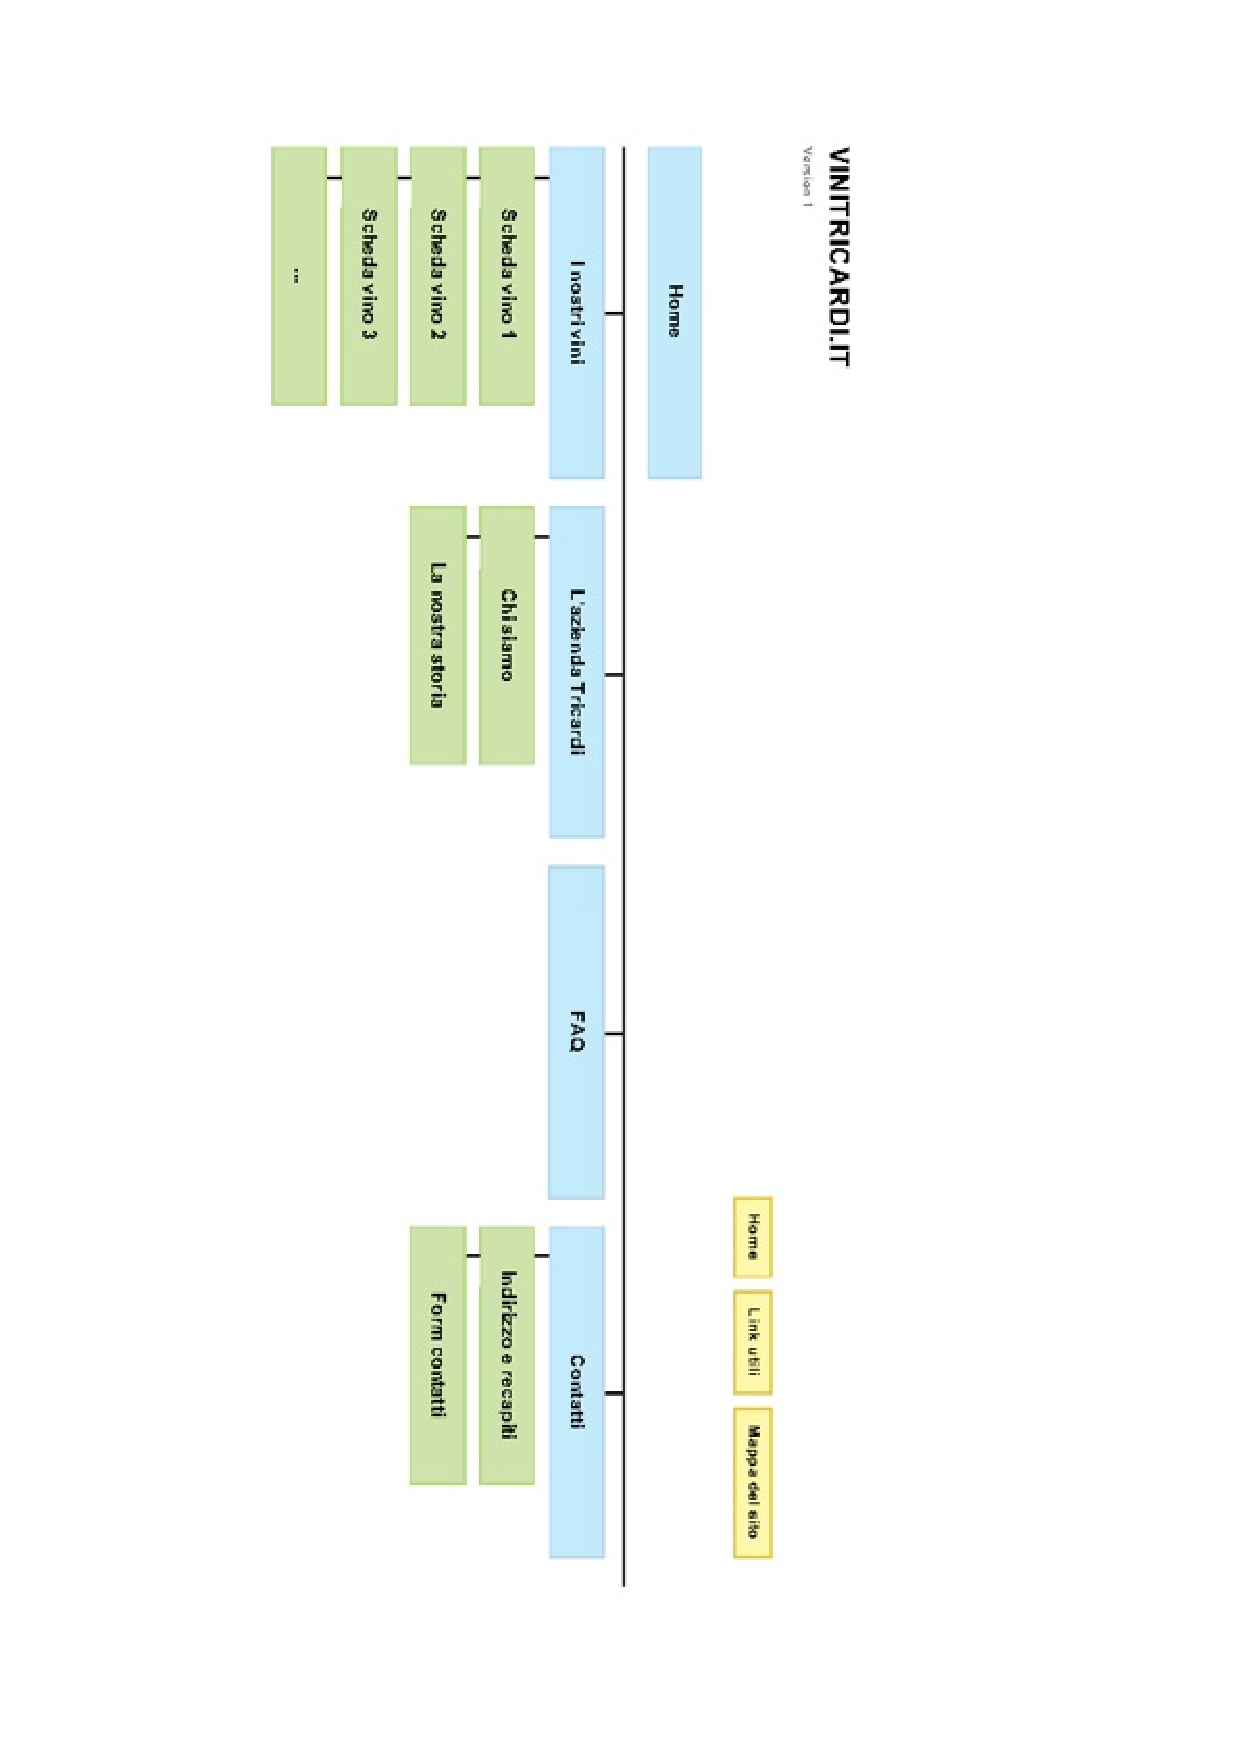
\includegraphics[scale=0.6]{mappa_del_sito_ver1.pdf}
\caption{Mappa del sito}\label{fig1}
\end{figure}

\chapter{Gabbia di massima delle pagine}
\begin{figure}
\centering
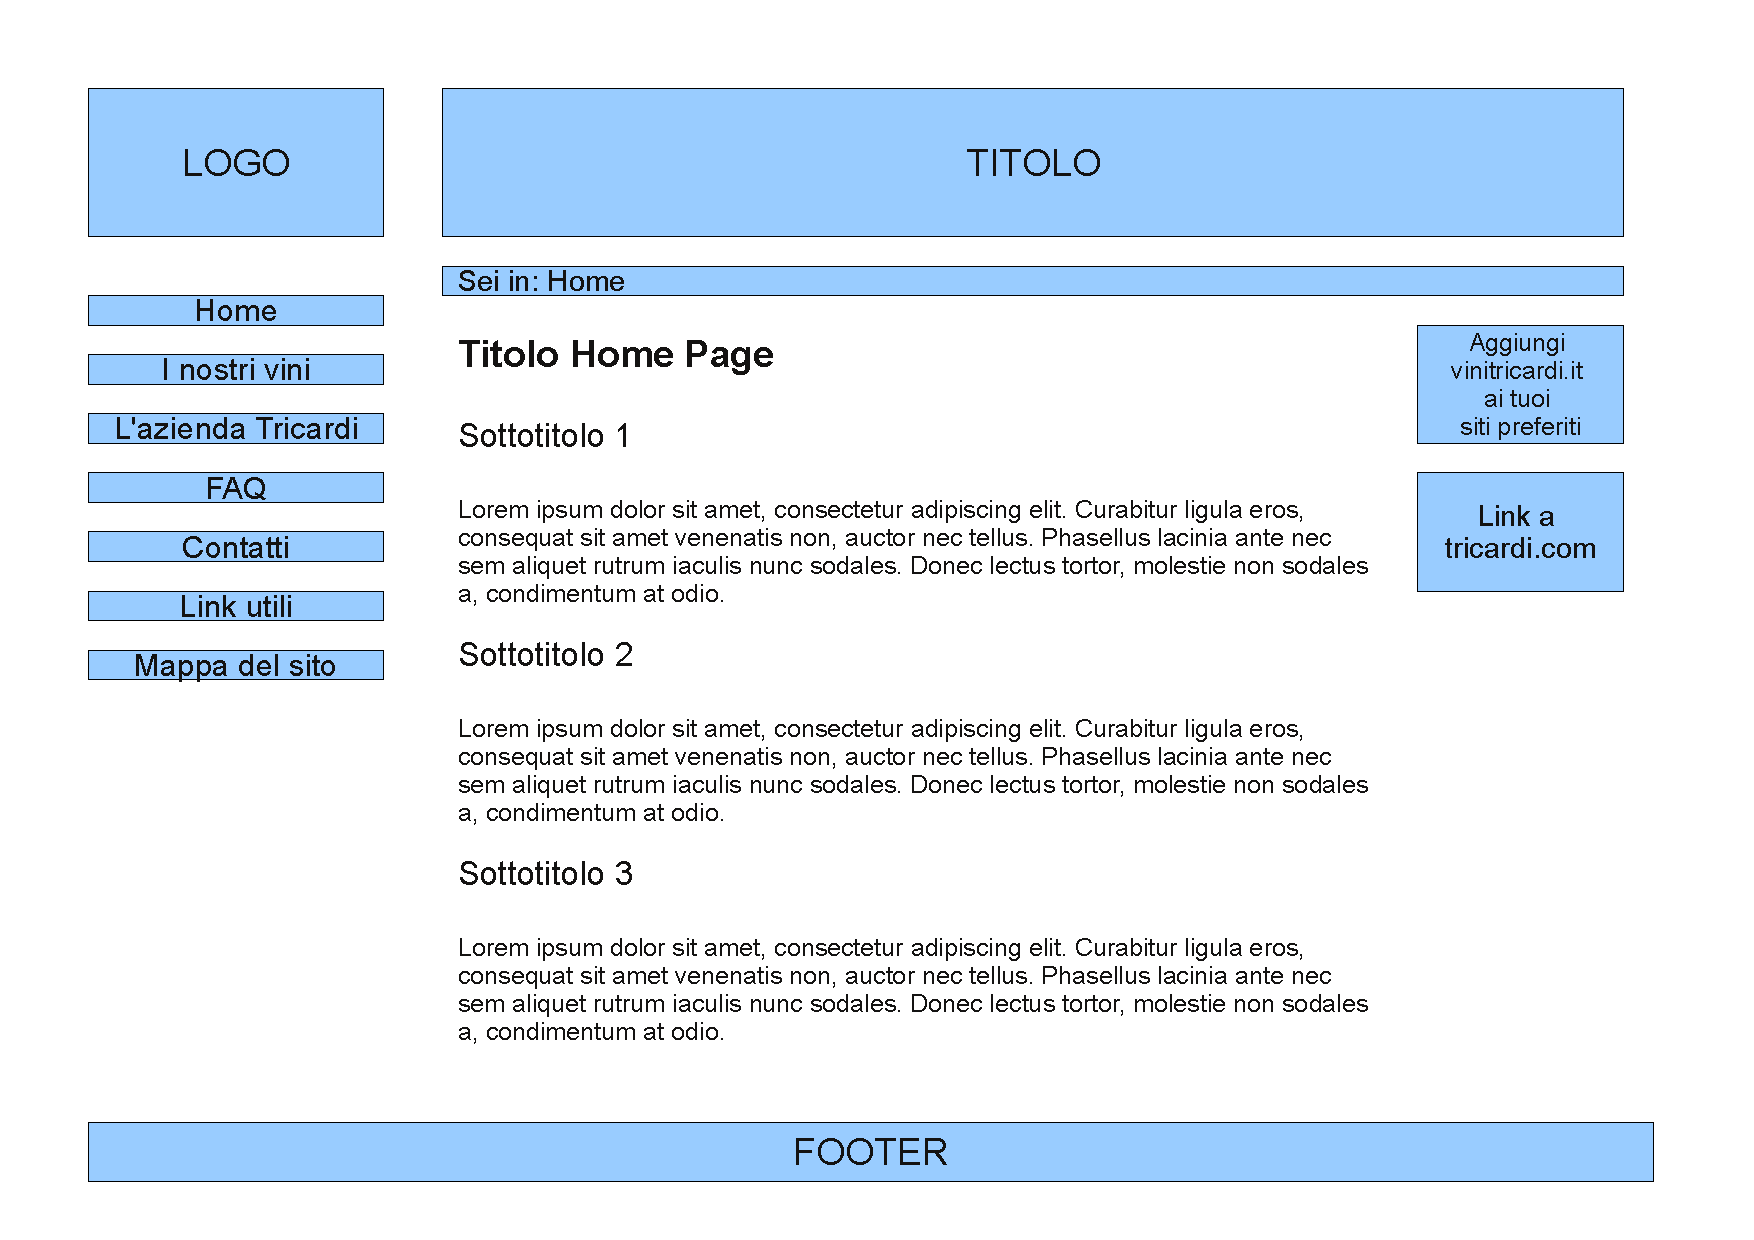
\includegraphics[scale=0.5]{gabbia_di_massima_home.pdf}
\caption{Gabbia di massima per la home page}\label{fig2}
\end{figure}
\begin{figure}
\centering
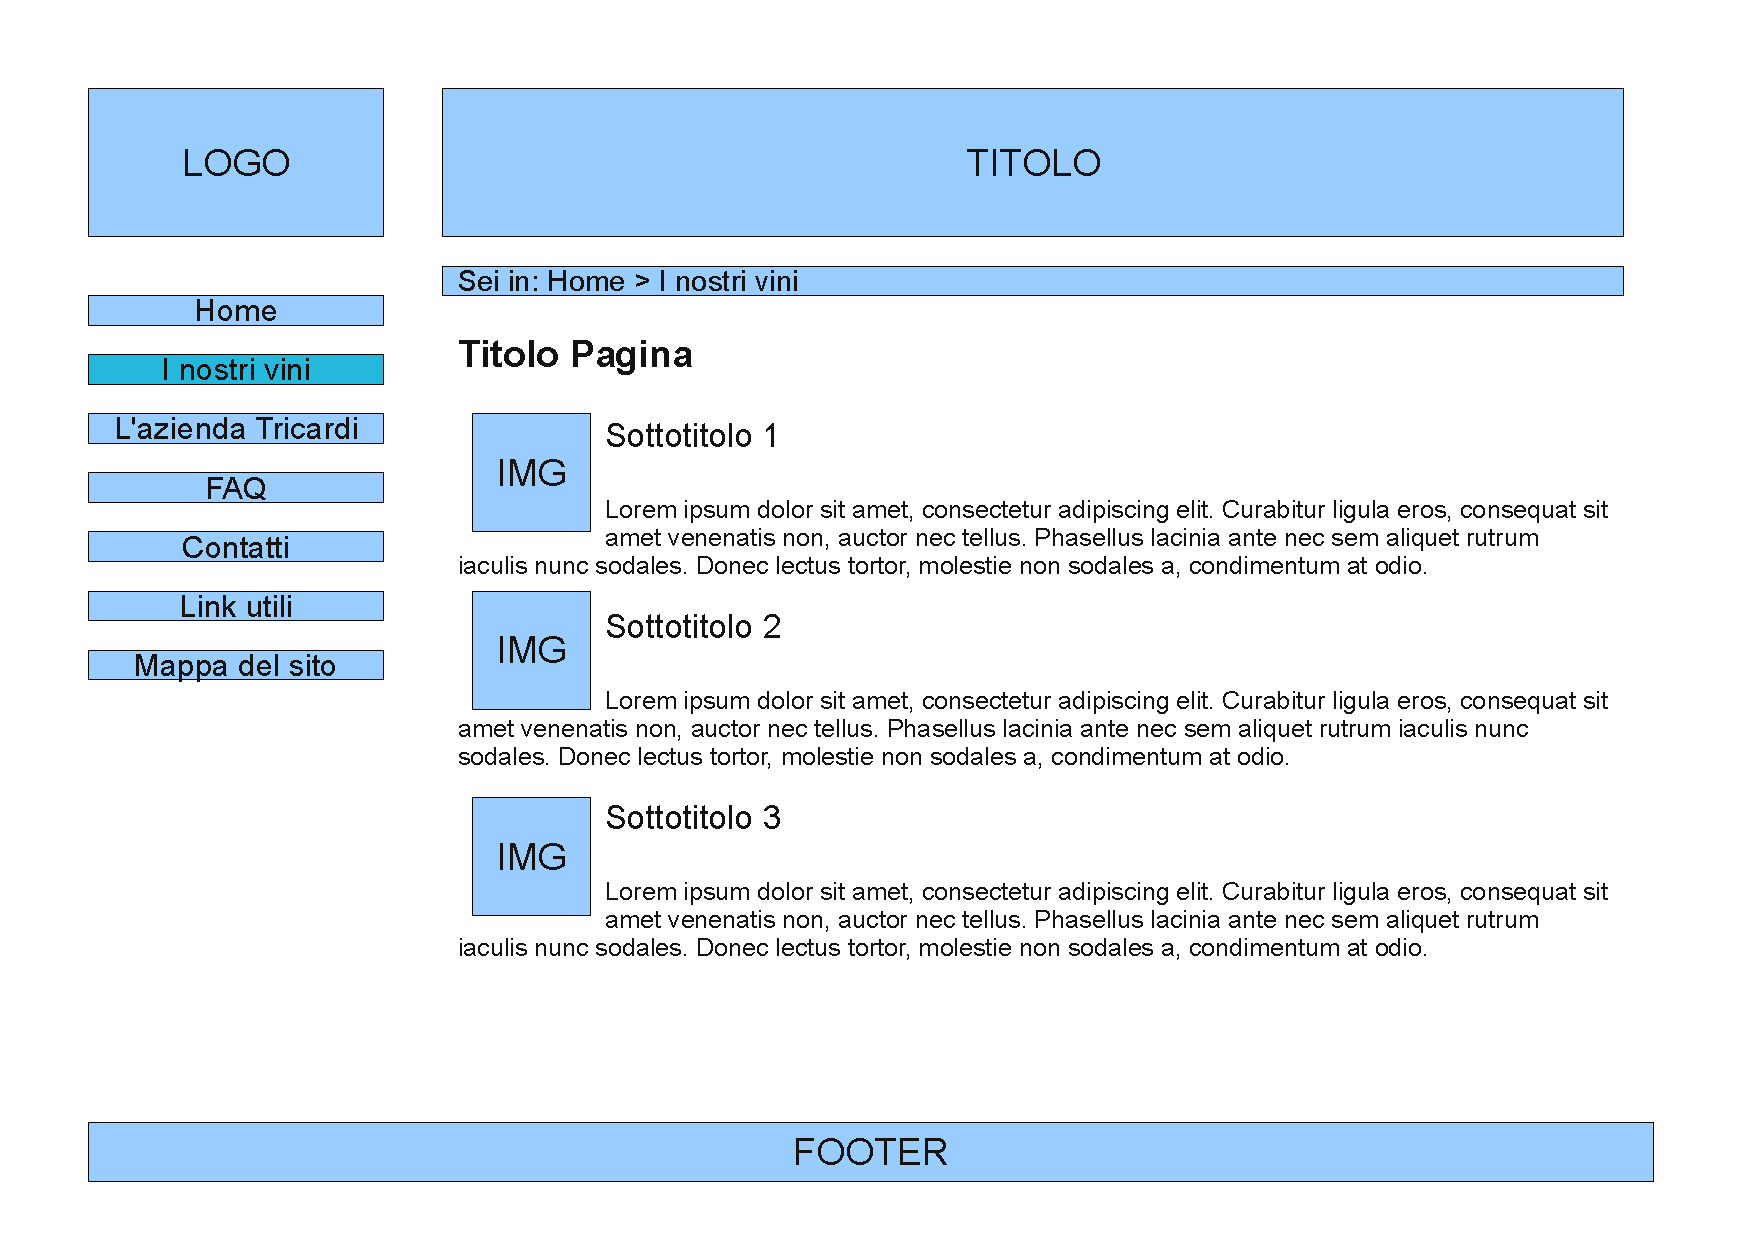
\includegraphics[scale=0.5]{gabbia_di_massima_page.pdf}
\caption{Gabbia di massima per una pagina di secondo livello}\label{fig3}
\end{figure}
\end{document}